\documentclass[11pt]{article}
% ----------------------- Paquetes -----------------------
\usepackage[spanish,es-noshorthands]{babel}
\usepackage[utf8]{inputenc}
\usepackage[T1]{fontenc}
\usepackage[margin=2cm]{geometry}
\usepackage{graphicx}
\usepackage{booktabs}
\usepackage{array}
\usepackage{longtable}
\usepackage{caption}
\usepackage{enumitem}
\usepackage{amsmath}
\usepackage{csquotes}
\usepackage{titlesec}
\usepackage{hyperref}

\usepackage[
  backend=biber,
  style=apa,
  natbib=true
]{biblatex}
\addbibresource{referencias.bib}

\hypersetup{
  colorlinks=true,
  linkcolor=black,
  citecolor=black,
  urlcolor=blue
}

% Optimización de espacios verticales
\setlist{noitemsep, topsep=2pt, parsep=0pt, partopsep=0pt}
\setlength{\floatsep}{8pt plus 2pt minus 2pt}
\setlength{\textfloatsep}{10pt plus 2pt minus 2pt}
\setlength{\intextsep}{8pt plus 2pt minus 2pt}

\title{%
  \textbf{Proyecto integrador: Detección de neumonía en radiografía de tórax mediante Transfer Learning}\\[0.3em]
  \large\textit{Replicación de la solución de Rahman et al. (2020) y enfocado a la población adulta latinoamericana}
}

\author{%
  Francy Umbarila \and Juan Delgado \and Andrés Escobar
}

\date{Bogotá, D.\,C. Agosto de 2026}

\begin{document}

% ----------------------- Portada -----------------------
\begin{titlepage}
\centering
\vspace{1cm}

{\large \textbf{UNIVERSIDAD EXTERNADO DE COLOMBIA}\par}
\vspace{0.3cm}
{\large Programa de Ciencia de Datos\par}
\vspace{2cm}

{\LARGE \textbf{Proyecto integrador: Detección de neumonía en radiografía de tórax mediante Transfer Learning}\par}
\vspace{0.5cm}
{\large \textit{Replicación de la solución de Rahman et al. (2020) y enfocado a la población adulta latinoamericana}\par}
\vspace{1.5cm}

{\large \textbf{Primera entrega: Fase 1}\par}
\vspace{0.2cm}
{\large Comprensión del artículo, problema local y línea base\par}
\vspace{2cm}

{\large \textbf{Integrantes}\par}
\vspace{0.2cm}
{\large Francy Umbarila \(\cdot\) Juan Delgado \(\cdot\) Andrés Escobar\par}
\vspace{1cm}

{\large Asignatura: Deep Learning \(\cdot\) Docente: Juliana De Mier Medellín\par}
\vspace{0.3cm}
{\large Link al repositorio: \href{https://github.com/6odoy/integrated_project}{Integrated Project}\par}

\vfill

{\large Bogotá, D.\,C. Agosto de 2026\par}

\end{titlepage}

\clearpage
\pagenumbering{arabic}

% =========================================================
\section{Comprensión y sustentación del artículo base}
% =========================================================

\subsection{El problema y por qué esta arquitectura y no otra}

Rahman et al. \parencite{rahman2020} automatizaron la detección de neumonía en radiografías de tórax y la diferenciación entre origen bacteriano y viral. Su enfoque prioriza la necesidad clínica: aunque la radiografía es la prueba de primera línea, su interpretación padece variabilidad interobservador y escasez de radiólogos en regiones con bajos recursos. Así, el objetivo es construir un sistema de apoyo al diagnóstico donde la métrica crítica es minimizar los falsos negativos.

La arquitectura empleada es una CNN preentrenada ajustada mediante Transfer Learning. Esta elección se sustenta en tres razones:

\textbf{(i)} La señal diagnóstica es una textura espacial local (opacidades alveolares en infecciones bacterianas e infiltrados intersticiales en virales). La convolución —con pesos compartidos y campo receptivo creciente— codifica esta estructura con invarianza a la traslación y eficiencia parametral.

\textbf{(ii)} Evita la extracción manual de descriptores de textura, la cual ha mostrado un desempeño inferior en estudios previos.

\textbf{(iii)} El dataset comprende 5.247 imágenes (órdenes de magnitud por debajo de lo requerido para entrenar desde cero); el aprendizaje por transferencia a partir de ImageNet es un requisito de viabilidad.

Los autores comparan cuatro redes (AlexNet, ResNet18, DenseNet201 y SqueezeNet), fundamentando la elección de la arquitectura en evidencia empírica.

\subsection{Supuestos que el artículo asume sin discutir}

\begin{itemize}
  \item \textbf{Verdad de terreno:} Asume que las etiquetas del expediente médico están libres de error, ignorando la variabilidad entre expertos.
  \item \textbf{Transferibilidad de ImageNet:} Presupone que filtros entrenados con imágenes RGB naturales se transfieren óptimamente a proyecciones en escala de grises.
  \item \textbf{Suficiencia de la imagen:} Asume que una proyección frontal es autosuficiente, prescindiendo de metadatos clínicos (edad, síntomas, laboratorios).
  \item \textbf{Plausibilidad del aumento:} Considera que rotaciones y traslaciones generan variabilidad clínicamente realista.
  \item \textbf{Representatividad:} Asume que el conjunto de prueba representa la población objetivo para tamizajes en contextos diversos.
\end{itemize}

\subsection{Resultados reportados}

DenseNet201 supera a las demás arquitecturas con 98\% de exactitud (99\% sensibilidad, 97\% especificidad, 0,98 AUC, 0,981 F1) en "Normal vs. Neumonía", 95\% en "Bacteriana vs. Viral" y 93,3\% en tres clases. La configuración común (Tabla~\ref{tab:config}) valida la comparación. La Figura~\ref{fig:metricas} evidencia la ventaja en sensibilidad de DenseNet201 frente al sesgo de SqueezeNet hacia la especificidad.

\begin{table}[h]
\centering
\small
\caption{Configuración de entrenamiento reportada por Rahman et al. (2020).}
\label{tab:config}
\begin{tabular}{@{}ll|ll@{}}
\toprule
\textbf{Elemento} & \textbf{Valor} & \textbf{Elemento} & \textbf{Valor} \\
\midrule
Software & MATLAB 2019a & Optimizador & Descenso del gradiente (SGD) \\
Redes & AlexNet, ResNet18, DenseNet201, SqueezeNet & Momentum & 0,9 \\
Resolución & 227\texttimes227 / 224\texttimes224 & Mini-batch & 16 \\
Augmentación & Rotación 315\textdegree, escala/traslación 10\% & Learning rate ($\eta$) & 0,0003 \\
Datos & 5.247 imágenes & K-Folds CV & 5 Folds \\
\bottomrule
\end{tabular}
\end{table}

\begin{figure}[h]
\centering
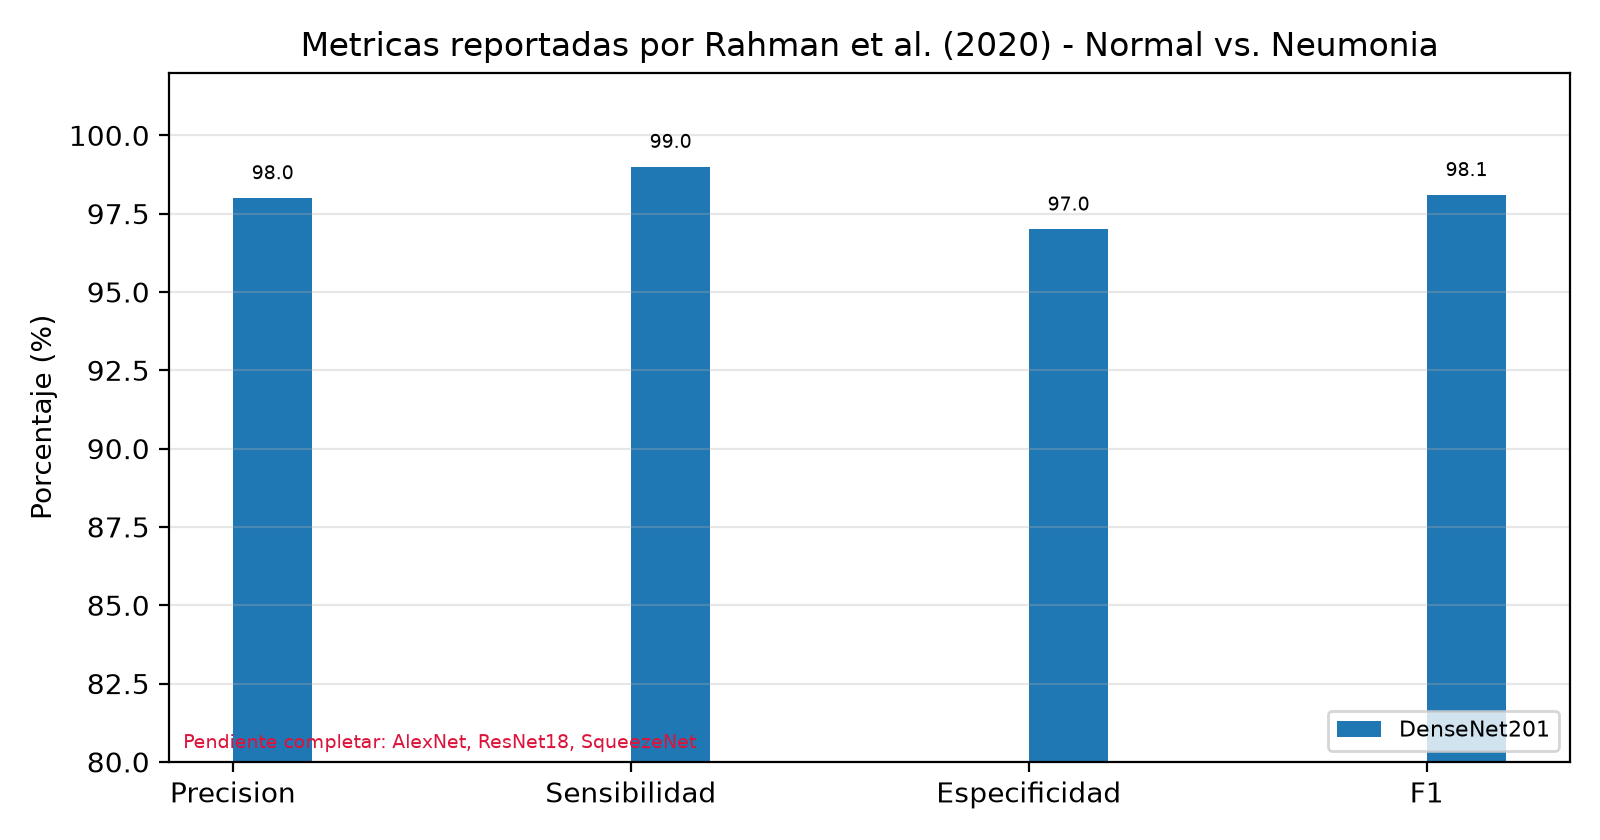
\includegraphics[width=0.55\textwidth]{figures/figura1.png}
\caption{Métricas reportadas por el artículo en la tarea normal frente a neumonía. Elaboración propia con datos de la Tabla 4 del artículo.}
\label{fig:metricas}
\end{figure}

\subsection{Limitantes encontrados}

Se identifican cuatro aspectos críticos que comprometen la replicabilidad del artículo:
\begin{itemize}
  \item \textbf{Trazabilidad de la partición:} No se especifica si el aumento de datos se aplicó tras la partición o si hubo separación por paciente, arriesgando fugas entre pliegues.
  \item \textbf{Evaluación dual:} Coexisten validación cruzada en 5 pliegues y un test set fijo de 419 imágenes, sin reportar varianza entre pliegues.
  \item \textbf{Ausencia de línea base e intervalos:} Falta comparación con modelos simples e intervalos de confianza para evaluar el aporte real de la profundidad.
  \item \textbf{Explicabilidad no analizada:} Los mapas de activación omiten verificar si la red aprende señales clínicas o atajos (marcas hospitalarias), riesgo documentado en la literatura \parencite{zech2018, degrave2021}. Mitigar este sesgo es el objetivo de la Fase 3.
\end{itemize}

\subsection{Qué podemos reproducir y qué debemos reducir}

El método es reproducible con datos e hiperparámetros públicos, aplicando cuatro reducciones justificadas:

\textbf{(i) Framework:} Traducción de MATLAB a TensorFlow/Keras (se busca convergencia comparable, no identidad numérica exacta).

\textbf{(ii) Sustitución de red:} SqueezeNet se adaptará o sustituirá por MobileNetV2 al no estar disponible nativamente en Keras.

\textbf{(iii) Cómputo:} Reducción de 20 ejecuciones a 3 muestras por configuración con partición fija, reportando media y desviación estándar.

\textbf{(iv) Parámetros:} Ajuste del batch size según disponibilidad de GPU manteniendo la resolución $224\times224$.

% =========================================================
\section{Planteamiento del problema local}
% =========================================================

\subsection{Pregunta, tarea y variable objetivo}

\textbf{Pregunta:} ¿Una CNN preentrenada y ajustada con el dataset pediátrico de Kermany conserva sensibilidad suficiente para priorizar el triaje al evaluarse en una población adulta latinoamericana (BRAX), superando a un baseline clásico bajo la misma partición?

\textbf{Tarea:} Clasificación binaria a nivel de imagen.

\textbf{Variable objetivo:} $y = 1$ ("Neumonía") vs. $y = 0$ ("Sin hallazgos").

\subsection{Relevancia en el contexto colombiano y latinoamericano}

La IRA es prioridad de vigilancia pública en Colombia. En la semana 38 de 2025, el INS reportó una mortalidad infantil por IRA de 4,3 por 100.000 \parencite{ins2025}. Aunque la radiografía está disponible, la lectura especializada es escasa fuera de las capitales.
El motivo epistémico de este proyecto no es sustituir el dataset del artículo por uno local; no existe un dataset colombiano etiquetado de acceso público comparable \parencite{kaushal2020}, sino auditar si un modelo entrenado bajo la misma distribución del artículo (pediatría, Guangzhou) generaliza a una población adulta y latinoamericana (BRAX, São Paulo) antes de considerar su uso en la región. Transferir modelos entrenados en pediatría asiática a urgencias latinoamericanas sin verificación representa un riesgo documentado \parencite{zech2018}; este proyecto cuantifica esa brecha en lugar de asumirla resuelta.

\subsection{Qué se conserva y qué se adapta}

Se conserva DenseNet201 \parencite{huang2017}, la transferencia de aprendizaje desde ImageNet, el preprocesamiento a $224 \times 224$, el dataset de entrenamiento (Kermany) y la sensibilidad como métrica principal. Adaptaciones respecto al artículo:
\begin{itemize}
  \item \textbf{Partición:} Estrictamente agrupada por paciente, corrigiendo el riesgo de fuga documentado en este dataset específico de Kaggle, en lugar de usar la partición train/test predefinida.
  \item \textbf{Evaluación de generalización:} Además del test interno de Kermany, el modelo se evalúa sin reentrenar sobre un subconjunto adulto de BRAX, para cuantificar la caída de desempeño al cambiar población, país y equipo de adquisición.
  \item \textbf{Métrica:} Se prioriza sensibilidad y AUPRC sobre "accuracy" en la evaluación externa, dado el cambio de prevalencia entre datasets.
  \item \textbf{Alcance:} Se mantiene el marco binario (Normal vs. Neumonía); no se replica la diferenciación bacteriana/viral por falta de etiqueta equivalente en BRAX.
\end{itemize}

% =========================================================
\section{Datos disponibles y sus limitaciones}
% =========================================================

\subsection{Conjunto de entrenamiento (Kermany) y conjunto de evaluación externa (BRAX)}

Se entrena con el mismo dataset del artículo: Kermany et al. \parencite{kermany2018} (Kaggle, Mooney 2018), 5.247 imágenes pediátricas de Guangzhou. Para evaluar la generalización a población adulta latinoamericana se utiliza BRAX \parencite{reis2022a, reis2022b} (PhysioNet), del Hospital Albert Einstein (São Paulo): se extrae un subconjunto con etiqueta CheXpert \parencite{irvin2019} de "Neumonía" positiva/negativa y proyección frontal, empleado exclusivamente como test externo, sin participar en el entrenamiento ni en la selección de hiperparámetros.

\textbf{Variable objetivo operativa:} Clase positiva ($y=1$): «Neumonía»; clase negativa ($y=0$): «Sin hallazgos». En BRAX, los casos ambiguos ($-1$) se excluyen de la evaluación externa.

\subsection{Particiones previstas y prevención de Data Leakage}

Sobre Kermany se descarta la partición train/test predefinida de Kaggle --fuente documentada de fuga entre pliegues cuando imágenes del mismo paciente aparecen en ambos conjuntos-- y se reconstruye una partición 70/15/15 estratificada por etiqueta a nivel de paciente (Tabla~\ref{tab:particiones}). Sobre BRAX se emplea el subconjunto elegible en su totalidad, únicamente como evaluación externa (0\% en entrenamiento o validación), preservando su prevalencia real. El desbalance en el entrenamiento con Kermany se maneja mediante weighted loss.

\begin{table}[h]
\centering
\small
\caption{Esquema de partición por paciente.}
\label{tab:particiones}
\begin{tabular}{@{}llp{7cm}@{}}
\toprule
\textbf{Partición} & \textbf{Prop.\ / Unidad} & \textbf{Función y regla de uso} \\
\midrule
Entrenamiento (Kermany) & 70\% $\cdot$ Pacientes & Ajuste de pesos. Partición aumentada y reequilibrada. \\
Validación (Kermany) & 15\% $\cdot$ Pacientes & Selección de hiperparámetros, early stopping y umbral de decisión. \\
Prueba (Kermany) & 15\% $\cdot$ Pacientes & Evaluación interna única en Fase 2. Conserva prevalencia real del dataset. \\
Evaluación externa (BRAX) & 100\% $\cdot$ Pacientes elegibles & Sin fuga por diseño (fuera del entrenamiento). Mide generalización a población adulta latinoamericana. \\
\bottomrule
\end{tabular}
\end{table}

\textbf{Alcance y limitaciones:} La partición sobre Kermany permite validación rigurosa sin fuga entre pliegues. La evaluación externa en BRAX tiene limitaciones propias:

(a) su etiqueta de "Neumonía" proviene de extracción NLP sobre informes radiológicos, no de verdad clínica confirmada

(b) al provenir de un único hospital privado paulista, no permite generalizar al sector público colombiano

(c) la edad está agrupada en quinquenios, impidiendo un análisis continuo

(d) los fabricantes de los equipos de adquisición están anonimizados. Se evaluará sobre un subconjunto representativo de BRAX según presupuesto computacional para la extracción y el cómputo.

\subsection{Estrategia de transferencia y distancia entre dominios}

Se empleará DenseNet201 (o DenseNet121). Se consideran dos brechas de dominio:
1. \textbf{ImageNet $\rightarrow$ Rayos X:} Los primeros bloques (bordes/texturas) transfieren bien; los superiores requieren ajuste fino parcial.
2. \textbf{Kermany (entrenamiento) $\rightarrow$ BRAX (evaluación externa):} Brecha no mitigada por fine-tuning; mide directamente la caída de desempeño esperable al desplegar el modelo en una población distinta a la de entrenamiento (pediátrico/Guangzhou vs.\ adulto/São Paulo). Se comparará el desempeño en BRAX frente al test interno de Kermany para cuantificar esta caída.

% =========================================================
\section{Línea base y plan de modelamiento}
% =========================================================

\subsection{Métrica principal y su justificación}

La métrica principal es la sensibilidad para «Neumonía» con especificidad $\ge 0,80$, junto con AUC-ROC y AUPRC. Refleja el costo asimétrico del error: un falso negativo retrasa el tratamiento y arriesga la vida; un falso positivo genera una revisión radiológica adicional. El umbral de decisión se fija exclusivamente en validación.

\subsection{Línea base construida}

Tres modelos con partición idéntica y semilla fija (42):

\textbf{(i)} Predictor trivial (clase mayoritaria).

\textbf{(ii)} Descriptores manuales (histograma de intensidad $128\times128$) + PCA + Regresión Logística / Random Forest.

\textbf{(iii)} Perceptrón Multicapa (MLP) de una capa oculta (64 unidades) sobre las mismas características.

\begin{table}[h]
\centering
\small
\caption{Rendimiento de referencia en prueba (intervalos de confianza 95\% vía 1.000 muestras bootstrap).}
\label{tab:baseline}
\begin{tabular}{@{}lccccc@{}}
\toprule
\textbf{Modelo} & \textbf{Sens.\ @esp\(\ge\)0,80} & \textbf{Especif.} & \textbf{AUC-ROC} & \textbf{AUPRC} & \textbf{F1} \\
\midrule
Trivial (clase mayoritaria) & 1,000 & 0,000 & 0,500 & 0,737 & 0,849 \\
Regresión logística + PCA & 0,732 & 0,751 & 0,802 & 0,923 & 0,804 \\
Random Forest & 0,938 & 0,755 & 0,947 & 0,981 & 0,927 \\
MLP mínimo (64 unidades) & 0,932 & 0,793 & 0,939 & 0,972 & 0,930 \\
\bottomrule
\end{tabular}
\end{table}

\subsection{Plan de modelamiento y criterio de justificación}

DenseNet201 preentrenado ($224 \times 224$), aumento en entrenamiento, Adam ($lr = 1\mathrm{e}{-4}$, ReduceLROnPlateau) y Weighted Binary Cross-Entropy. EarlyStopping por AUC de validación (paciencia 5) sobre 3 semillas.

La arquitectura profunda se justificará si y solo si cumple cuatro condiciones:
\begin{itemize}
  \item \textbf{Magnitud:} Sensibilidad al menos 5\% superior al mejor baseline (intervalos bootstrap 95\% no solapados).
  \item \textbf{Estabilidad:} Ventaja consistente en las tres semillas.
  \item \textbf{Costo:} Tiempo de inferencia viable en entorno clínico.
  \item \textbf{Auditoría:} Mapas Grad-CAM \parencite{selvaraju2017} focalizados en el parénquima pulmonar y no en artefactos o marcas hospitalarias.
\end{itemize}

\subsection{Riesgos}

Contingencia ante retrasos en el acceso a PhysioNet: se usará PadChest (BIMCV, Valencia; adultos, español) como conjunto de evaluación externa alternativo. El riesgo computacional se mitiga con el subconjunto reducido, precisión mixta y DenseNet121.

\begin{figure}[h]
\centering
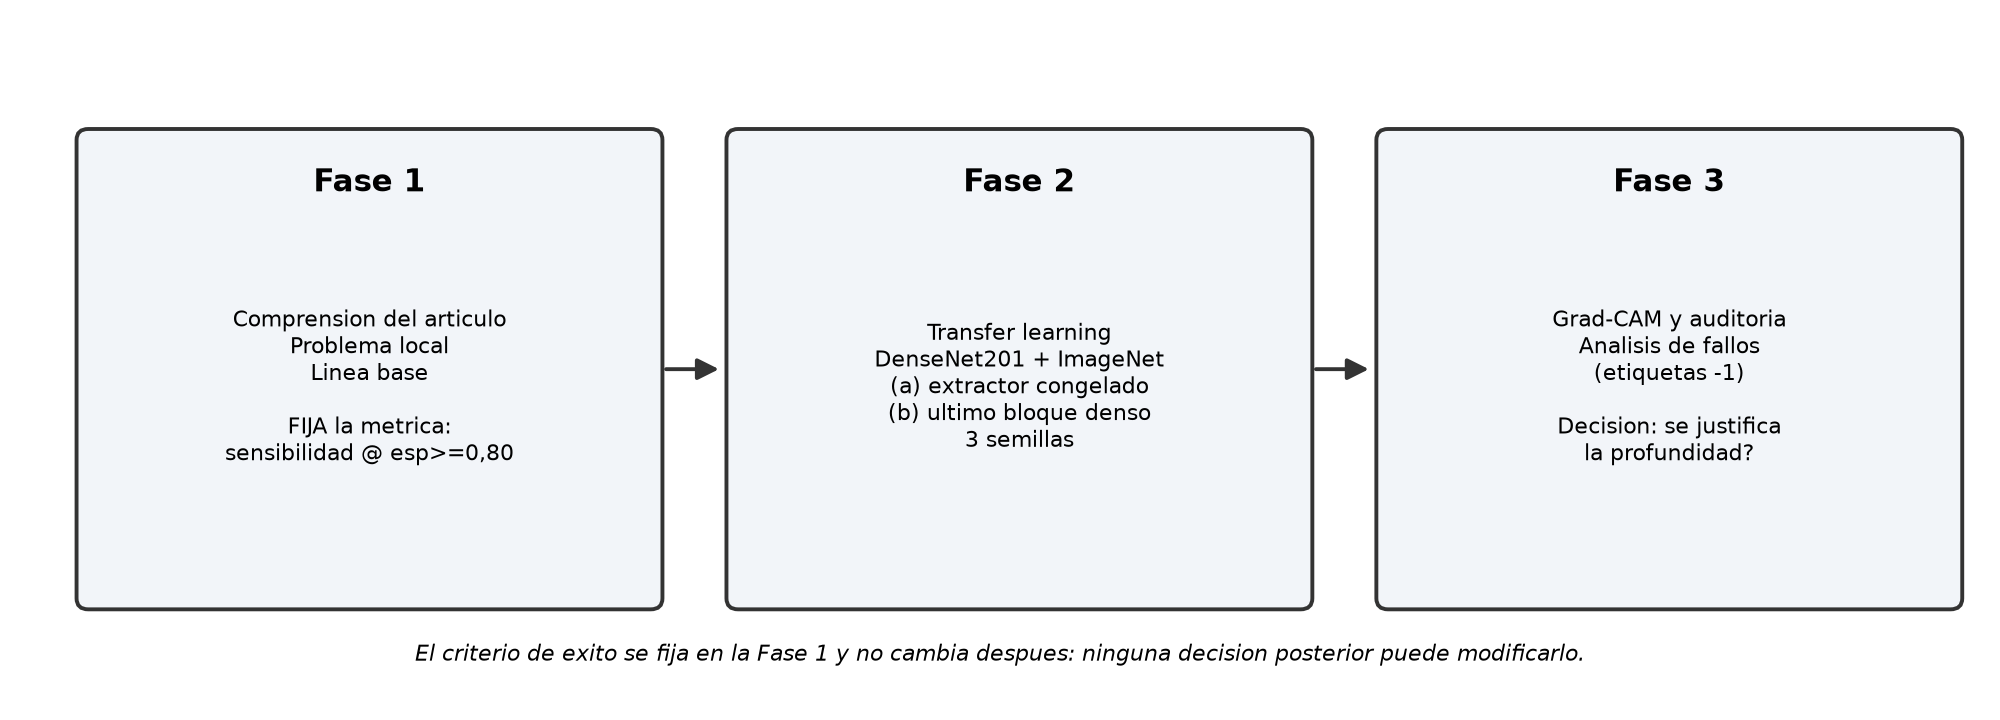
\includegraphics[width=0.55\textwidth]{figures/figura2.png}
\caption{Secuencia metodológica en tres fases.}
\label{fig:fases}
\end{figure}

% =========================================================
\section{Declaración de uso de IA}
% =========================================================

El equipo empleó herramientas de IA generativa como apoyo en la redacción y revisión del código; todas las decisiones técnicas y analíticas fueron verificadas y asumidas plenamente por los integrantes.

\printbibliography[title={Referencias}]

\end{document}